\documentclass[12pt]{exam}
\usepackage[utf8]{inputenc}

\usepackage[margin=1in]{geometry}
\usepackage{amsmath,amssymb}
\usepackage{multicol}
\usepackage{tikz}
\usepackage{tikz-3dplot}


\newcommand{\class}{SA 405}
\newcommand{\term}{Fall 2018}
\newcommand{\examnum}{Test 1 Sample Questions}
\newcommand{\examdate}{}
\newcommand{\timelimit}{}

\pagestyle{head}
\firstpageheader{}{}{}
\runningheader{\class}{\examnum\ - Page \thepage\ of \numpages}{\examdate}
\runningheadrule


\begin{document}

\noindent
\begin{tabular*}{\textwidth}{l @{\extracolsep{\fill}} r @{\extracolsep{6pt}} r}
\textbf{\class} & \textbf{Name:} & \makebox[2in]{\hrulefill}\\
\textbf{\term} &&\\
\textbf{\examnum} &&\\
%\textbf{\examdate} &&\\
\end{tabular*}
%%\textbf{Time Limit: \timelimit} & Teaching Assistant & \makebox[2in]{\hrulefill}
%\end{tabular*}\\
%\rule[2ex]{\textwidth}{2pt}
%
%\begin{itemize}
%\item Do {\bf not} write your name on each page, only write your name above.
%
%\item No books or notes % or calculators
%% that do symbolic manipulation (such as TI-89 or TI-92) 
% are allowed. %{\bf One} 8.5 by 11 inch formula/note sheet is allowed.
%
%\item You may use your calculator on this test.
%
%\item Show all work clearly. (Little or no credit will be given for a numerical
%answer without the correct accompanying work.
%Partial credit is given where appropriate.) 
%
%\item If you need more space than is provided, use the back of the previous page. 
%
%\item Please read the question carefully.
%If you are not sure what a question is
%asking, ask for clarification.
%
%\item If you start over on a problem, please CLEARLY indicate what your final
%  answer is, along with its accompanying work.
%
%\item All formulations must have descriptions of any indices, parameters, and decision variables used. All constraints must be described. 
%\end{itemize}
%
%
%\begin{center}
%Grade Table (for teacher use only)\\
%\addpoints
%\gradetable[v][questions]
%\end{center}
%
%\noindent
%\rule[2ex]{\textwidth}{2pt}
%
%
%
%\vspace{0.2cm}
%
%
%
%\newpage

\begin{questions}



%%%%%%%%
\question[20] Consider the directed network shown below, where the numbers on the arcs represent cost, $c_{ij}$, to send one unit of flow along the arc.  Use the start of a formulation given below to answer the following questions.

\begin{center}
        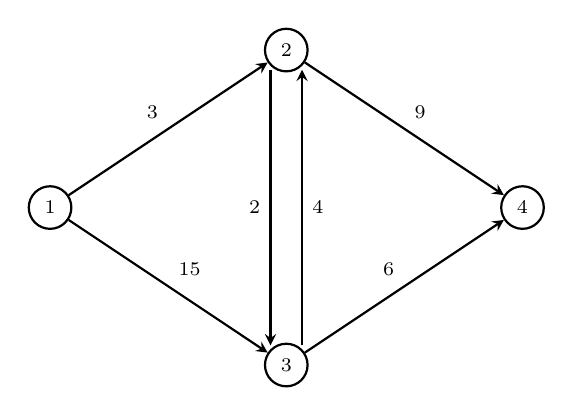
\begin{tikzpicture}
          [font=\scriptsize,
          node/.style={shape=circle,draw=black,fill=white!20, text=black,minimum width=0.5cm,thick},
          arc/.style={->,>=stealth,thick},
          edge/.style={thick}]
          
            \node (1) [node] at (0,0) {1};
            \node (2) [node] at (3,2) {2};
            \node (3) [node] at (3,-2) {3};
            \node (4) [node] at (6,0) {4};
%          \node[label={\small $b_1$=1}] (1) at (0,0) {1};
%            \node[label={\small $b_2$=0}] (2) at (3,2) {2};
%            \node (3) at (3,-2) [label=below:{$b_3=0$}]{3};
%            \node[label={\small $b_4$=-1}] (4) at (6,0) {4};
% 
          \coordinate (A2) at (2.8,1.75);
          \coordinate (A3) at (2.8,-1.75);
          \coordinate (B2) at (3.2,1.75);
          \coordinate (B3) at (3.2,-1.75);
          
          \draw [arc] (1) to node [auto] {3} (2);
            \draw [arc] (1) to node [auto] {15} (3);
            \draw [arc] (A2) to node [left] {2} (A3);
            \draw [arc] (B3) to node [right] {4} (B2);
            \draw [arc] (2) to node [auto] {9} (4);
            \draw [arc] (3) to node [auto] {6} (4);

        \end{tikzpicture}
\end{center}



\noindent\underline{Indices}
\begin{tabbing}


\hspace{.5cm} \= $N :=$ \hspace{.5cm} \= set of nodes, $i$ \\
\> $A :=$ \> set of directed arcs $(i,j)$ from node $i$ to node $j$, for some $i$ and $j$ in $N$ \\

\noindent\underline{Data}\\% [units]\\
\> $c_{ij} :=$ \> cost to flow one unit from node $i$ to node $j$, for $(i,j) \in A$ \\

\noindent\underline{Decision Variables}\\% [units]\\
\> $x_{ij} := $ \> number of units of flow on arc $(i,j)$, for $(i,j) \in A$  \\
\end{tabbing}

\begin{parts}

\part
We  place one unit of supply at node 1, 1 unit of demand at node 4 and zero units of supply at all other nodes. Formulate an objective function to compute the minimum cost strategy for meeting the demand at node 4. 

% \[
%    \begin{array}{llll}
%      \displaystyle\min_{ \tiny{\it X}} &  3 X_{12} + 15 X_{13} + 2 X_{23} + 4 X_{32} + 9 X_{24} + 6 X_{34} & &  \\
%    \end{array}
%\]
%
%or
%
% \[
%    \begin{array}{llll}
%      \displaystyle\min_{ \tiny{\it X}} &  \sum\limits_{(i,j) \in A} c_{ij} X_{ij} & &  \\
%    \end{array}
%\]
%
%\vfill
\part What two classes of network problems does this one belong to?

\part Label all four nodes in the network diagram above with their ``net supply'' or $b_i$ value.


%\vspace{0.5cm}
%
%See the labels on the figure above.  Note that there is one unit of supply at node 1, one unit of demand at node 4, and nodes 2 and 3 are transshipment nodes.

\part Write the constraints for this problem using concrete form.

\part Write the constraints for this problem using abstract form.

% \[
%    \begin{array}{llll}
%
%& X_{32} + X_{34} - X_{13} - X_{23} = 0 & & {\rm (BOF, Node~3)}\\
%    \end{array}
%    \]
%
%\vfill

\part Find the optimal objective value by inspection, and write the corresponding values of the decision variables for this solution.

%An optimal solution to the model shown is $X_{12}=X_{23}=X_{34}=1, ~ X_{13}=X_{32}=X_{24} = 0$, which gives an optimal objective value of 11.
\vfill

\end{parts}


%%%%%%%%%%%%%%%%%%5
\newpage

\question
US NorthWest plans to install fiber in a metro area network that is expected to experience increased demand due to the opening of a large manufacturing facility.  The Central Offices (COs) in the network are represented by vertices in the graph below.  The edges in the graph represent the possible fiber paths linking the COs.  The number on edge $(i,j)$ represents the cost $c_{ij}$ (in \$1000) of installing fiber between COs $i$ and $j$.

\begin{center}
\includegraphics[width = .4\textwidth]{uswest_network}
\end{center}

Network planners developed the following partial integer program to solve for the collection of edges that will minimize the cost of connecting all the central offices in the network via a fiber spanning tree.  (Let $V$ represent the set of vertices in the graph.  Let $E$ represent the set of edges in the graph.)

\begin{equation}
  \label{eq:mst}
  \tag{MST}
  \begin{array}{llll}
    \min & \displaystyle \sum_{(i,j)\in E} c_{ij} X_{ij} & & \\
    \mbox{s.t.} & \sum_{j:(i,j) \in E} X_{ij} + 
    \sum_{j:(j,i) \in E} X_{ji} \geq 1, & \forall i \in V &
    \mbox{(a)} \\[4mm]
    & \sum_{(i,j) \in E} X_{ij} = ~? & & \mbox{(b)} \\[4mm]
    &  t \sum_{\substack{i,j \in V' \\ (i,j) \in E}} X_{ij} \leq |V'| - 1 & \forall V' \subseteq V & \mbox{(c)} \\[4mm]
    & X_{ij} \in \{0,1\} & \forall (i,j) \in E. &
  \end{array}
\end{equation}



\begin{parts}
  

\part Write the concrete form of constraint type (a) from \eqref{eq:mst} for vertex 4. What is the purpose of this constraint?

%\[  \sum_{j:(4,j) \in E} X_{4j} +  \sum_{j:(j,4) \in E} X_{j4} \ge 1 \]
%or
%\[ X_{45} + X_{47} + X_{24} + X_{23} \ge 1 \]
%
%This constraint ensures that vertex 4 is connected to at least one other node.
%\vfill

%\part What GUSEK code would implement the objective function? Assume that $c$, $X$ and $E$ have already been defined for you.  
%
%\begin{verbatim}
%minimize obj:sum{(i,j) in E} c[i,j] * X[i,j];
%\end{verbatim}
%\vfill

%\newpage

\part Architect Ima Klutz spilled cappuccino on the formulation rendering the right hand side of constraint (b) illegible.  What is the purpose of constraint (b), and what should the missing number be?

%\[  \sum_{(i,j) \in E} X_{ij} = n-1 = 6 \]
%
%The purpose of this constraint is to ensure we have $n-1$ edges in our tree that contains $n$ nodes.
%\vfill

\part The modeling team learns that city ordinances require that if link $(3,7)$ is built, then neither $(1,2)$ nor $(3,4)$ may be built.  Write a constraint to model this new requirement.

%\[ 2 - 2 X_{37} \ge X_{12} + X_{34} \]
%
%
%We can derive this constraint from the rule that says that when we want to model the constraint ``(binary variable) $Y = 1$ implies $f \leq 0$'' we use  $f \leq M(1-Y)$ where $M$ is a constant chosen so that $f \leq M$ always holds. Here the variable $X_{37}$ plays the role of $Y$ and requiring that $X_{12} = 0$ and $X_{34}=0$ is the same as requiring that $X_{12}+X_{34} \leq 0$, so $X_{12}+X_{34}$ plays the role of $f$. The quantity $f$ is clearly always less than 2 so we can take $M = 2$. This gives the answer above. 
%
%\vfill

\part The Central Office represented by vertex 3 is centrally located, but the equipment there is outdated.  If vertex 3 is used as a hub, meaning three or more fiber paths meet at vertex 3, the Central Office there will require a \$25,000 upgrade.  The modeling team adds a new binary variable $Y$ that indicates whether or not vertex 3 is used as a hub in the network design.  They modify the objective function by adding the term $25*Y$.  Write a constraint that forces $Y$ to be 1 if three or more selected edges connect to vertex 3.

%\[ X_{13} + X_{23} + X_{34} + X_{36} + X_{37} \le 3 Y + 2 \]
%
%We obtain this solution as follows. First we see that we want to impose the condition ``$X_{13} + X_{23} + X_{34} + X_{36} + X_{37} \geq 3$ implies $Y=1$''. This is logically equivalent to the condition that $Y = 0$ implies that $X_{13} + X_{23} + X_{34} + X_{36} + X_{37} \leq 2$. We'd like to use the rule mentioned in part (d) but our assumption is that $Y=0$, not $Y=1$. To fix this we introduce the variable $Z = 1-Y$. Now $Y=0$ precisely when $Z=1$, so we are trying to model ``$Z=1$ implies $X_{13} + X_{23} + X_{34} + X_{36} + X_{37} -2 \leq 0$''. This can be done using the rule with $f = X_{13} + X_{23} + X_{34} + X_{36} + X_{37} -2$ and $M = 3.$ We get 
%\[ X_{13} + X_{23} + X_{34} + X_{36} + X_{37} -2 \leq 3(1-Z), \]
%and substituting $Z = 1-Y$ we get 
%\[ X_{13} + X_{23} + X_{34} + X_{36} + X_{37} -2 \leq 3Y, \]
%which is equivalent to the condition that we gave as the answer above. 
%
%\vfill

\end{parts}



\end{questions}

\end{document}

